\documentclass{beamer}
\usepackage{ctex, hyperref}
\usepackage[T1]{fontenc}
\usepackage{caption}
% other packages
\usepackage{latexsym,amsmath,xcolor,multicol,booktabs,calligra,threeparttable,geometry,adjustbox,makecell}
\usepackage{graphicx,pstricks,listings,stackengine}

\author{刘斌 \inst{1} 甄洋 \inst{1} 李小帆 \inst{2}}
\title{
    规制融合对数字贸易的影响:\\
    基于WIOD数字内容行业的检验
}
\institute{
    \inst{1} 对外经济贸易大学中国WTO研究院, \\
    \inst{2} 复旦大学世界经济系
}
\usepackage{Whu}

% defs
\def\cmd#1{\texttt{\color{red}\footnotesize $\backslash$#1}}
\def\env#1{\texttt{\color{blue}\footnotesize #1}}
\definecolor{deepblue}{rgb}{0,0,0.5}
\definecolor{deepred}{rgb}{0.6,0,0}
\definecolor{deepgreen}{rgb}{0,0.5,0}
\definecolor{halfgray}{gray}{0.55}

\lstset{
    basicstyle=\ttfamily\small,
    keywordstyle=\bfseries\color{deepblue},
    emphstyle=\ttfamily\color{deepred},    % Custom highlighting style
    stringstyle=\color{deepgreen},
    numbers=left,
    numberstyle=\small\color{halfgray},
    rulesepcolor=\color{red!20!green!20!blue!20},
    frame=shadowbox,
}

\setCJKfamilyfont{zhsong}{simsun.ttc}
\setCJKfamilyfont{zhhei}{simhei.ttf}
\newcommand{\zhsong}{\CJKfamily{zhsong}}  %中易宋体
\newcommand{\zhhei}{\CJKfamily{zhhei}}  %中易黑体

\begin{document}

\kaishu

\begin{frame}
    \titlepage
    \vfill
    \begin{center}
        \small
        吴予锐 \  2022302111417
    \end{center}
\end{frame}

\begin{frame}
    \begin{multicols}{2}
    \tableofcontents[
        sections={1-4},
        sectionstyle=show,
        subsectionstyle=show/shaded/hide,
        subsubsectionstyle=show/shaded/hide
    ]
    \columnbreak
    \tableofcontents[
        sections={5-8},
        sectionstyle=show,
        subsectionstyle=show/shaded/hide,
        subsubsectionstyle=show/shaded/hide
    ]
    \end{multicols}
\end{frame}


\section{研究背景}
\begin{frame}{研究背景}
    \centering
    \large
    \begin{itemize}
        \item 全球数字贸易高速增长。
        \item 数字贸易目前没有形成全球统一规则。
        \item 世界各经济体所主张的数字贸易规则并不一致。
    \end{itemize}
\end{frame}

\begin{frame}{研究动机}
    \begin{itemize}
        \item 较少文献研究数字贸易条款经济影响,且与数字贸易相关的文献大多仅限于政策分析和定性研究。 {\zhhei 本文较早关注规制融合与数字贸易的相关性的经验研究。}
        \item 囿于数据可获性,数字贸易的度量一直是学术界的难点。 {\zhhei 本文为计量分析提供可供检验的“干净样本”。}
        \item 国内对数字贸易规则深度的研究较少。 {\zhhei 本文对规制融合进行了较为准确的测度。} 国内外对美式和欧式模板的经验研究较少。 {\zhhei 本文构建数字贸易模板相似度指标分析二者对数字贸易影响的差异性。}
        \item 传统分析侧重规制融合通过降低贸易成本促进国际贸易。 {\zhhei 本文选取双边网络效应进行数字贸易机制分析。}
    \end{itemize}
\end{frame}


\section{研究问题}
\begin{frame}{研究问题}
    \centering
    \large
    \begin{itemize}
        \item 在全球数字贸易规则尚不完善的背景下,规制融合对数字贸易存在怎样的影响?
    \end{itemize}
\end{frame}


\section{研究内容}
\begin{frame}{研究过程}
    \begin{enumerate}
        \item 基准回归
        \begin{itemize}
            \item {\footnotesize 采用普通最小二乘回归和泊松伪极大似然估计方法进行基准回归分析}
            \item {\footnotesize 更换数字指标进行稳健性检验}
            \item {\footnotesize 采用多期倍差方法解决样本选择偏差产生的内生性问题;采用工具变量法和两阶段最小二乘方法解决模型中的反向因果问题}
        \end{itemize}
        \item 机制检验
        \begin{itemize}
            \item {\footnotesize 构建中介效应模型采用间接测度法进行普通最小二乘回归对贸易成本进行机制检验}
            \item {\footnotesize 运用双边双向网络链接作为替代变量进行中介效用分析对双边网络效应进行机制检验}
            \item {\footnotesize 运用政治制度和经济制度测算出双边制度距离对制度距离进行机制检验}
        \end{itemize}
        \item 扩展分析
        \begin{itemize}
            \item {\footnotesize 对3个数字贸易行业进行分样本回归以分析数字贸易行业的差异性}
            \item {\footnotesize 构建数字贸易美式模板相似度指标和数字贸易欧式模板相似度指标进行回归以分析美式模板与欧式模板的差异性}
        \end{itemize}
    \end{enumerate}
\end{frame}

\begin{frame}{研究发现}
    \begin{enumerate}
        \item 规制融合对数字贸易具有促进作用
        \item 规制融合对数字贸易可能的影响渠道
        \begin{itemize}
            \item 数字贸易通过降低贸易成本促进数字贸易的发展
            \item 规制融合通过增强双边网络效应进而促进数字贸易的发展
            \item 规制融合会通过降低制度距离促进数字贸易的发展
        \end{itemize}
        \item 规制融合对不同数字贸易行业产生的影响
        \begin{itemize}
            \item 对“电影、视频和电视节目制作,录音和音乐出版活动以及节目编制和广播活动”行业的数字贸易作用最大且最为显著
            \item 其次是“电信业”
            \item 最后是“计算机编程、咨询等相关活动与信息服务活动”行业
        \end{itemize}
        \item 尽管美式模板的标准更高,但相较于欧式模板,美式模板并没有表现出对数字贸易更强的促进作用
    \end{enumerate}
\end{frame}


\section{文献综述}
\begin{frame}
    \setbeamertemplate{itemize subitem}{}
    \begin{itemize}
        \item 区域贸易协定对“第一代”和“第二代”贸易的影响
        \begin{itemize}
            \item Viner(1950); Cernat(2001); 韩剑等(2018); Horn et al.(2010);盛斌和果婷(2016).
        \end{itemize}
        \item 数字贸易的概念与测定
        \begin{itemize}
            \item Weber(2010); OECD(2017).
        \end{itemize}
        \item 数字技术对传统货物贸易和服务贸易的影响
        \begin{itemize}
            \item Freund and Weinhold(2004); Choi(2010); 裴长洪和刘斌(2020); Lendle et al.(2016); Kim et al.(2017); Javier and Janos(2018).
        \end{itemize}
        \item 数字贸易规则对数字贸易的影响
        \begin{itemize}
            \item Sacha(2003); Weber(2010); 李杨等(2016); 周念利和陈寰琦(2018).
        \end{itemize}
    \end{itemize}
\end{frame}


\section{理论模型}
\begin{frame}{基本假定}
    \textbf{模型的基本假定为:}
    \begin{enumerate}
        \item 数字产品市场为垄断竞争市场,数字产品之间为不完全替代关系,替代弹性为 $\sigma$ 
        \item 每个企业 $v$ 只生产 $1$ 种数字产品,生产的产品可以同时向国内和国外市场出售
        \item $i$ 国企业进入 $j$ 国市场需要支付固定成本 $F_{ij}$ 
        \begin{itemize}
            \item 固定成本的存在使各国向其他国家或地区出口数字产品的数量由零利润条件内生决定
        \end{itemize}
        \item 劳动是企业唯一的生产投入要素,生产函数具有常数规模报酬属性
    \end{enumerate}
\end{frame}

\begin{frame}{数字贸易的需求与偏好}
    \begin{itemize}
        \item 使用垄断竞争的Dixit-Stiglitz模型和不变替代弹性(CES)效用函数可以表示\underline{数字产品进口国 $j$ 的代表性消费者的偏好}% 为:
        \begin{gather*}
            U_j = (\sum_{i=1}^{R} \sum_{v=1}^{n_i} x_{vij}^{\frac{\sigma - 1} {\sigma}})^{\frac{\sigma -1}{\sigma}} \tag{1}
        \end{gather*}
        \begin{itemize}
            \item $i, j, v$ 分别为出口国,进口国和数字贸易企业(或者产品种类)
            \item $n_i$ 代表企业数量
            \item $R$ 代表出口国数量
            \item $X_{vij}$ 代表 $j$ 国从 $i$ 国进口的数字产品 $v$ 的数量
            \item $\sigma$ 表示差异化的数字产品替代弹性( $\sigma > 1$ )
        \end{itemize}
    \end{itemize}
\end{frame}

\begin{frame}{数字贸易的需求与偏好}
    \begin{itemize}
        \item \underline{数字产品进口国 $j$ 的代表性消费者的预算约束}% 为:
        \begin{gather*}
            P_jY_j = \sum_{i=1}^{R} \sum_{v=1}^{n_i} P_{vij}X_{vij} \tag{2}
        \end{gather*}
        \begin{itemize}
            \item $Y_j$ 代表 $j$ 国的实际收入水平
            \item $P_j$ 代表消费者在最优消费决策情况下面临的最终价格指数
            \item $P_{vij}$ 代表 $j$ 国从 $i$ 国进口 $v$ 种类数字产品的价格
        \end{itemize}
    \end{itemize}
\end{frame}

\begin{frame}{数字贸易的需求与偏好}
    \begin{itemize}
        \item 通过 (1) 和 (2) 两式,可得 \underline{$j$ 国数字产品价格指数和数字产品的需求函数}% 为:
        \begin{align*}
            P_j &= (\sum_{i=1}^{R} \sum_{v=1}^{n_i} P_{vij}^{1 - \sigma})^{\frac{\sigma - 1}{\sigma}} \tag{3} \\
            X_{vij} &= (\frac{P_{vij}}{P_j})^{-\sigma}Y_j,\quad \forall v, i \tag{4}
        \end{align*}
    \end{itemize}
\end{frame}

\begin{frame}{数字贸易的供给与成本}
    \begin{itemize}
        \item $i$ 国 $v$ 企业的成本函数和利润函数
        \begin{align}
            C_{vij} &= w_i l_{vij} = w_i(\beta X_{vij} + F_{ij}) \tag{5} \\
            \pi_{vi} &= \sum_{j=1}^{R} \pi_{vij} = \sum_{j=1}^{R} [P_{cij X_{vij} - w_i(\beta X_{vij} + F_{ij})}] \tag{6}
        \end{align}
        \begin{itemize}
            \item $C_{vij}$ 代表 $i$ 国企业 $v$ 将产品出口到 $j$ 国时面临的成本
            \item $F_{ij}$ 表示出口国 $i$ 的每家企业进入到进口国 $j$ 的固定成本
            \item $w_i$ $i$ 国工资水平
            \item $\beta$ 反映生产的可变成本(即每单位数字产品的生产需要 $\beta$ 单位的劳动)
            \item $w_i \beta X_{vij}$ 可变劳动成本
            \begin{itemize} 
                \item $\beta X_{vij}$ 表示 $i$ 国企业 $v$ 生产 $X_{vij}$ 件数字产品时需要的劳动量
            \end{itemize}
            \item $w_i F_{ij}$ 固定成本,受规制融合影响
            \item $\pi_{vi}$ 代表 $i$ 国企业 $v$ 获取的利润
        \end{itemize}
    \end{itemize}
\end{frame}

\begin{frame}{数字贸易的供给与成本}
    \begin{itemize}
        \item 在 CES 效用函数下的垄断竞争市场,利润最大化时产品的销售价格等于边际成本乘以固定价格加成
        \begin{align}
            P_{vij}^{*} = \frac{\sigma}{\sigma - 1} \beta w_i \tag{7}
        \end{align}
    \end{itemize}
\end{frame}

\begin{frame}{数字贸易的供给与成本}
    \begin{itemize}
        \item 产量
        \begin{align}
            X_{vij}^{*} = \frac{(\sigma - 1) F_{ij}}{\beta} \tag{8}
        \end{align}
    \end{itemize}
\end{frame}

\begin{frame}{规制融合对数字贸易的影响}
    \begin{itemize}
        \item 当达到市场均衡时,每个数字贸易市场的需求等于供给
        \item $X_{ij}=n_i X_{vij};\ P_{vij}=P_{ij};\ P_{j}=(\sum_{i=1}^R n_iP_{ij}^{1-\sigma}){\frac{1}{1-\sigma}}$
        \begin{align}
            \frac{(\sigma - 1)F_{ij}}{\beta} = \frac{(\sum_{i=1}^R n_iP_{ij}^{1-\sigma}){\frac{1}{1-\sigma}}}{P_{ij}^{\sigma}} Y_j \tag{9}
        \end{align}
    \end{itemize}
\end{frame}

\begin{frame}{规制融合对数字贸易的影响}
    \begin{itemize}
        \item 当数字贸易市场均衡时,$i$ 国的出口企业数量 $n_i$ 对 $F_{ij}$ 求导
        \begin{gather*}
            \frac{{\mathrm{d}n_i}}{{\mathrm{d}F_{ij}}} = \frac{(1-\sigma)n_i}{\sigma F_{ij}\varpi_{ij}} < 0 \tag{10} \\
            \text{如果} \sigma > 1 \quad \text{且} \varpi_{ij}=\frac{n_iP_{ij}^{1-\sigma}}{\sum_{i=1}^R n_i P_{ij}^{1-\sigma}} \leqslant 1
        \end{gather*}
        \begin{itemize}
            \item $\varpi_{ij}$ 代表 $i$ 在 $j$ 国价格指数中所占份额
        \end{itemize}
    \end{itemize}
\end{frame}

\begin{frame}{规制融合对数字贸易的影响}
    \begin{itemize}
        \item 当数字贸易市场均衡时,$i$ 和 $j$ 国的数字贸易量 $X_{ij}$ 对 $i$ 与 $j$ 国的固定成本 $F_{ij}$ 求导
        \begin{gather*}
            \frac{\mathrm{d}X_{ij}}{\mathrm{d}F_{ij}} = \frac{X_{ij}n_i}{F_{ij}}\left(1+\frac{1-\sigma}{\sigma \varpi_{ij}}\right)<0 \quad \text{如果} \quad \sigma(1-\varpi_{ij})>1 \tag{11}
        \end{gather*}
    \end{itemize}
\end{frame}

\section{数据来源}
\begin{frame}{数字贸易:基于数字交付服务的出口额分析}
    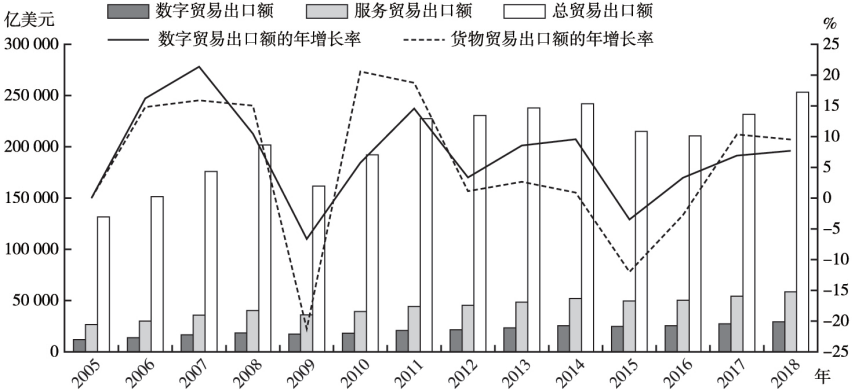
\includegraphics[width=\textwidth]{pic/Fig1.png}
    \begin{center}
        \text{ 图1 \quad 2005-2018年全球数字贸易出口额及其年增长情况 }
    \end{center}
\end{frame}

\begin{frame}{规制融合}
    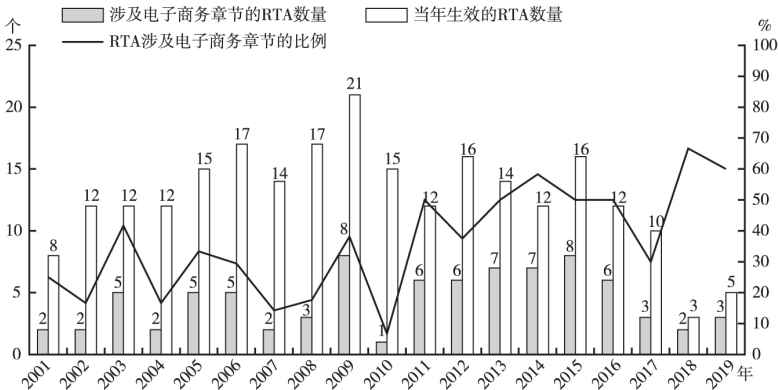
\includegraphics[width=\textwidth]{pic/Fig2.png}
    \begin{center}
        \text{ 图2 \quad 2001-2019年涉及电子商务章节的RTA统计情况 }
    \end{center}
\end{frame}

\begin{frame}{规制融合}
    \begin{center}
        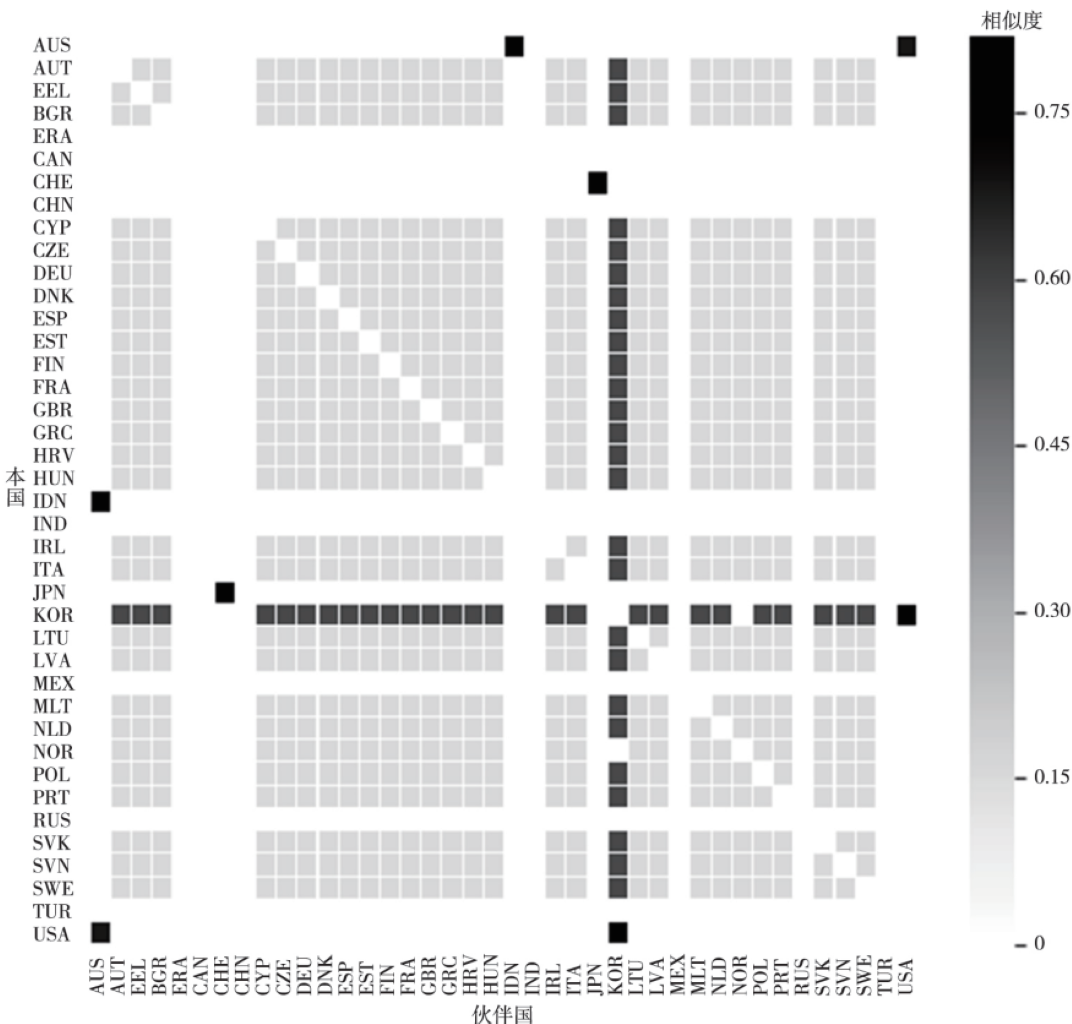
\includegraphics[height=0.8\textheight, keepaspectratio]{pic/Fig3.png}
        \text{ 图3 \quad 2014年国家间达成数字贸易规则的美式模板相似度统计 }
    \end{center}
\end{frame}


\section{实证分析}
\subsection{计量模型}
\begin{frame}{计量模型的建立}
    \begin{itemize}
        \item 引力模型
        \begin{gather*}
            RDT_{ijkt} = \beta_0 + \beta_1 Rule_{ijt} + \beta Controls + v_i + v_j + v_k + v_t + \epsilon_{ijkt} \tag{12}
        \end{gather*}
        \begin{itemize}
            \item $i$ 代表本国
            \item $j$ 代表贸易伙伴国
            \item $k$ 代表行业
            \item $t$ 代表年份
            \item $RDT_{ijkt}$ 被解释变量,国 $i$ 和贸易伙伴国 $j$ 在 $t$ 时期 $k$ 行业的数字贸易额占总贸易额的比重
            \item $Rule_{ijt}$ 解释变量,本国 $i$ 和贸易伙伴国 $j$ 在 $t$ 时期的规制融合水平
            \item $Controls$ 控制变量
            \item $v_i$ 本国固定效应
            \item $v_j$ 贸易伙伴国固定效应
            \item $v_k$ 年份固定效应
            \item $\epsilon_{ijkt}$ 随机干扰项
        \end{itemize}
    \end{itemize}
\end{frame}

\begin{frame}{核心指标度量}
    \begin{itemize}
        \item 核心被解释变量
        \begin{align*}
            RDT_{ijkt}
        \end{align*}
        \begin{itemize}
            \item 代表数字贸易
            \item $i$ 和 $j$ 国 $k$ 行业 $t$ 时期数字贸易额占总贸易额的比重
            \item 3 个具有数字贸易典型特征行业
            \begin{itemize}
                \item 电影、视频和电视节目制作,录音和音乐出版活动以及节目编制和广播活动
                \item 计算机编程、咨询等相关活动与信息服务活动
                \item 电信业
            \end{itemize}
            \item 4维层面数据
            \begin{itemize}
                \item 本国-贸易伙伴国-行业-年份
            \end{itemize}
        \end{itemize}
    \end{itemize}
\end{frame}

\begin{frame}{核心指标度量}
    \begin{itemize}
        \item 核心解释变量
        \begin{align*}
            Rule_{ijt}
        \end{align*}
        \begin{itemize}
            \item 代表规制融合
            \item 已签署的RTA是否含有电子商务等数字贸易章节定义经济体之间的规制融合
            \item 如果含有该章节(在生效之后),则取值为1,否则为0
            \begin{itemize}
                \item 1-6月生效的协定算作该年的数字贸易协定
                \item 7-12月生效的协定算作次年的数字贸易协定
            \end{itemize}
            \item “国家对”层面数据
        \end{itemize}
    \end{itemize}
\end{frame}

\begin{frame}{核心指标度量}
    \begin{itemize}
        \item 控制变量
        \begin{enumerate}
            \item $GDP_{it} \text{、} GDP_{jt}$
                \begin{itemize}
                    \item 本国、贸易伙伴国国内生产总值 
                \end{itemize}
            \item $Dist_{ij}$
            \begin{itemize}
                \item 双边地理距离 
            \end{itemize}
            \item $Contig_{ij}$
            \begin{itemize}
                \item 是否接壤
            \end{itemize}
            \item $Comlang_{ij}$
            \begin{itemize}
                \item 是否具有共同语言 
            \end{itemize}
            \item $Col_{ij}$
            \begin{itemize}
                \item 是否具有殖民关系 
            \end{itemize}
            \item $DoC_{ij}$
            \begin{itemize}
                \item 双边文化距离 
            \end{itemize}
            \item $Internet_{it}、Internet_{jt}$
            \begin{itemize}
                \item 本国和贸易伙伴国互联网水平 
            \end{itemize}
        \end{enumerate}
    \end{itemize}
\end{frame}

\subsection{基准回归}
\begin{frame}{基准回归分析}
    \scriptsize
    \centering
    \resizebox{\textheight}{!}{ 
        \begin{threeparttable}
        \caption{基准回归结果}
        \begin{tabular}{lcccccc}
        \toprule
         & \multicolumn{3}{c}{OLS} & \multicolumn{3}{c}{PPML} \\
        % \cmidrule(lr){2-4} \cmidrule(lr){5-7}
         & (1) & (2) & (3) & (4) & (5) & (6) \\
        \midrule
        $Rule_{ij}$ & 0.0018*** & 0.0024*** & 0.0026*** & 0.2682*** & 0.3544*** & 0.3877*** \\
         & (0.0002) & (0.0003) & (0.0003) & (0.0294) & (0.0441) & (0.0455) \\
        $GDP_{it}$ & & -0.0004*** & -0.0004*** & & -0.0539*** & -0.0579*** \\
         & & (0.0001) & (0.0001) & & (0.0119) & (0.0119) \\
        $GDP_{jt}$ & & -0.0004*** & -0.0004*** & & -0.0514*** & -0.0660*** \\
         & & (0.0001) & (0.0001) & & (0.0122) & (0.0117) \\
        $Dist_{ij}$ & & 0.0007*** & 0.0008*** & & 0.0992*** & 0.1096*** \\
         & & (0.0001) & (0.0001) & & (0.0190) & (0.0200) \\
        $Contig_{ij}$ & & -0.0026*** & -0.0027*** & & -0.5080*** & -0.5164*** \\
         & & (0.0002) & (0.0002) & & (0.0450) & (0.0463) \\
        $Comlang_{ij}$ & & 0.0059*** & 0.0064*** & & 0.8050*** & 0.8535*** \\
         & & (0.0008) & (0.0008) & & (0.0766) & (0.0767) \\
         $Col_{ij}$ & & -0.0020*** & -0.0017*** & & -0.4007*** & -0.3662*** \\
         & & (0.0003) & (0.0003) & & (0.0615) & (0.0632) \\
        $DoC_{ij}$ & & & -0.0002*** & & & -0.0309*** \\
         & & & (0.0001) & & & (0.0107) \\
        $Internet_{it}$ & & & -0.0002 & & & -0.0390 \\
         & & & (0.0002) & & & (0.0302) \\
        $Internet_{jt}$ & & & -0.0003* & & & -0.0503* \\
         & & & (0.0002) & & & (0.0291) \\
        常数项 & 0.0064*** & 0.0182*** & 0.0210*** & -5.1082*** & -3.3779*** & -2.8428*** \\
         & (0.0005) & (0.0028) & (0.0027) & (0.0768) & (0.4228) & (0.4189) \\
        观测值 & 35 100 & 35 100 & 33 100 & 35 100 & 35 100 & 33 003 \\
        $R^2$ & 0.0153 & 0.0227 & 0.0238 & 0.0111 & 0.0163 & 0.0164 \\
        \bottomrule
        \end{tabular}
        \begin{tablenotes}
        \item \textit{说明:} 括号内的值为稳健标准误,* 、**、***分别表示估计系数在 10\% 、5\% 和 1\% 的水平上显著,如未做特殊说明,则所有回归都控制了本国、贸易伙伴国、行业以及年份固定效应,后表同。
        \end{tablenotes}
        \end{threeparttable}
    }
\end{frame}

\begin{frame}{基准回归分析}
    \begin{itemize}
        \item 第(1)-(3)列进行普通最小二乘回归(OLS);第(4)-(6)列使用泊松伪极大似然估计(PPML)进行回归
    \end{itemize}
\end{frame}

\begin{frame}{稳健性检验}
    \vspace{-0.5cm}
    \tiny
    \setlength{\tabcolsep}{3pt}
    \centering
    \begin{threeparttable}
    \captionsetup{font=tiny}
    \caption{稳健性检验-重新度量数字贸易指标}
    \renewcommand{\arraystretch}{0.8} % 减小行距
    \begin{tabular}{lcc}
    \toprule
    & \multicolumn{1}{c}{(1)} & \multicolumn{1}{c}{(1)} \\
    \midrule
    $Rule_{ij}$ & 0.5453*** & 0.5142*** \\
    & (0.0600) & (0.0606) \\
    $GDP_i$ & 0.8073*** & 0.8047*** \\
    & (0.0176) & (0.0190) \\
    $GDP_j$ & 0.8039*** & 0.7995*** \\
    & (0.0183) & (0.0197) \\
    $Dist_{ij}$ & -0.6122*** & -0.6266*** \\
    & (0.0229) & (0.0217) \\
    $Contig_{ij}$ & -0.4286*** & -0.4269*** \\
    & (0.0623) & (0.0657) \\
    $Comlang_{ij}$ & 1.1633*** & 1.1286*** \\
    & (0.0788) & (0.0885) \\
    $Col_{ij}$ & -0.1264 & -0.1190 \\
    & (0.0925) & (0.0932) \\
    $DoC_{ij}$ & & -0.0313** \\
    & & (0.0159) \\
    $Internet_i$ & & -0.0062 \\
    & & (0.0645) \\
    $Internet_j$ & & 0.0147 \\
    & & (0.0607) \\
    常数项 & -36.5401*** & -36.1791*** \\
    & (0.7777) & (0.8190) \\
    观测值 & 35100 & 33003 \\
    $R^2$ & 0.6220 & 0.6155 \\
    \bottomrule
    \end{tabular}
    \end{threeparttable}
\end{frame}

\begin{frame}{稳健性检验}
    \begin{table}
        \centering
        \caption{更换规制融合指标}
        \label{tab:robustness_check}
        \begin{tabular}{lccc}
            \toprule
            & (1) & (2) & (3) \\
            \midrule
            $RWords_{gt}$ & 0.2045*** & 0.2814*** & 0.2999*** \\
             & (0.0206) & (0.0289) & (0.0293) \\
            控制变量 & 控制 & 控制 & 控制 \\
            观测值 & 35,100 & 35,100 & 33,003 \\
            R$^2$ & 0.0113 & 0.0166 & 0.0167 \\
            \bottomrule
        \end{tabular}
    \end{table}
\end{frame}

\begin{frame}{内生性问题的讨论与处理}
    \begin{itemize}
        \item DID 模型
        \begin{gather*}
            RDT_{zt}=\phi_0+\phi_1 DID_{zt}+\phi Controls+v_z+v_t+\epsilon_{zt} \tag{13}
        \end{gather*}
        \begin{itemize}
            \item $DID_{zt}$ 表示因个体而异的处理期虚拟变量
            \begin{itemize}
                \item 若个体 $z$ 在 $t$ 期接受处理代表进入处理期,此后时期均取值为 $1$,否则为 $0$
                \item 等价于处理组虚拟变量 $treat_z$ 和处理期虚拟变量 $post_t$ 的交乘项
            \end{itemize}
            \item $v_z$ 表示个体固定效应
            \item $v_t$ 表示年份固定效应
            \item $\epsilon_{zt}$ 为随机干扰项
        \end{itemize}
    \end{itemize}    
\end{frame}

\begin{frame}{内生性问题的讨论与处理}
    \begin{table}
        \centering
        \caption{多期倍差法(DID)的回归结果}
        \label{tab:DID_results}
        \begin{tabular}{lccc}
            \toprule
            & (1) & (2) & (3) \\
            \midrule
            DID$_{zt}$ & 0.0040*** & 0.0049*** & 0.0053*** \\
                       & (0.0003)  & (0.0004)  & (0.0004)  \\
            控制变量   & 控制      & 控制      & 控制      \\
            个体固定效应 & 控制      & 控制      & 控制      \\
            年份固定效应 & 控制      & 控制      & 控制      \\
            观测值     & 35,100    & 35,100    & 33,003    \\
            R$^{2}$    & 0.0060    & 0.0135    & 0.0142    \\
            \bottomrule
        \end{tabular}
    \end{table}
\end{frame}

\begin{frame}{内生性问题的讨论与处理}
    \scriptsize
    \centering
    \resizebox{\textwidth}{!}{
        \begin{threeparttable}
            \caption{两阶段最小二乘法的估计结果}
            \label{tab:two_stage_least_squares}
            \begin{tabular}{lcccccc}
                \toprule
                % & \multicolumn{1}{c}{工具变量是 “两国实现规制融合的概率值”} & \multicolumn{1}{c}{工具变量是 “两国实现规制融合的概率值 $\times$ 年份”} & \multicolumn{1}{c}{工具变量是 “两国到赤道距离差取自然对数后的倒数”} & \multicolumn{1}{c}{工具变量是 “两国到赤道距离差取自然对数后的倒数 $\times$ 年份”} & \multicolumn{1}{c}{同时引入(1)和(3)两个工具变量} & \multicolumn{1}{c}{同时引入(2)和(4)两个工具变量} \\
                & \makecell[c]{工具变量是 \\ “两国实现 \\ 规制融合的 \\ 概率值”} 
                & \makecell[c]{工具变量是 \\ “两国实现规 \\ 制融合的概 \\ 率值 $\times$ 年份”} 
                & \makecell[c]{工具变量是 \\ “两国到赤道 \\ 距离差取 \\ 自然对数 \\ 后的倒数”} 
                & \makecell[c]{工具变量是 \\ “两国到赤道 \\ 距离差取自 \\ 然对数后的 \\ 倒数 $\times$ 年份”} 
                & \makecell[c]{同时引入 \\ (1) 和 (3) \\ 两个工具 \\ 变量} 
                & \makecell[c]{同时引入 \\ (2) 和 (4) \\ 两个工具 \\ 变量} \\
                % \cmidrule(lr){2-3} \cmidrule(lr){4-5} \cmidrule(lr){6-7}
                & (1) & (2) & (3) & (4) & (5) & (6) \\
                \midrule
                $Rule_{ijt}$ & 0.0102*** & 0.0102*** & 0.0087*** & 0.0087*** & 0.0102*** & 0.0102*** \\
                & (0.0004) & (0.0004) & (0.0017) & (0.0017) & (0.0004) & (0.0004)  \\
                控制变量 & 控制 & 控制 & 控制 & 控制 & 控制 & 控制 \\
                \makecell[c]{Kleibergen-Paap \\ rk LM 统计量} & 5534.5713 & 5521.7264 & 68.9331 & 68.9375 & 5650.6850 & 5637.7088 \\
                & [0.000] & [0.000] & [0.000] & [0.000] & [0.000] & [0.000] \\
                \makecell[c]{Kleibergen-Paap \\ rk Wald F 统计量} & 20525.1132 & 20369.2289 & 300.3013 & 300.4280 & 10426.9758 & 10348.1463 \\
                & \{16.38\} & \{16.38\} & \{16.38\} & \{16.38\} & \{19.93\} & \{19.93\} \\
                \makecell[c]{Hansen-Overid \\ 统计量} & & & & & 0.7286 & 0.7632 \\
                & & & & & [0.3933] & [0.3823] \\
                观测值 & 33,003 & 33,003 & 33,003 & 33,003 & 33,003 & 33,003 \\
                R$^2$  & 0.0069 & 0.0068 & 0.0128 & 0.0128 & 0.0070 & 0.0069 \\
                \bottomrule
            \end{tabular}
            \begin{tablenotes}
                \item {\zhhei 说明:} 小括号内的值为稳健标准误;中括号内的值为相应统计量的 P 值;大括号内的值为 Stock-Yogo 检验 10\%水平上的临界值。Kleibergen-Paap rk LM 统计量检验工具变量与内生变量的相关性,报告的是 LM 统计量及其 P 值,拒绝原假设是合理的;Kleibergen-Paap rk Wald F 统计量检验工具变量是否为弱识别,报告的是 F 统计量及其 10\% 水平下的临界值,超过临界值是合理的。Hansen-Overid 是过度识别检验,报告的是 chi2 统计量及其 P 值,不拒绝原假设是合理的。
            \end{tablenotes}
        \end{threeparttable}
    }
\end{frame}

\subsection{机制检验}
\begin{frame}{机制检验}
    \begin{itemize}
        \item 中介效应模型
        \begin{tiny}
        \begin{gather*}
            M=\gamma_0+\gamma_1 Rule_{ijt}+\gamma Controls+v_i+v_j+v_k+v_t+\epsilon_{ijkt} \tag{14} \\
            RDT_{ijkt}=\omega_0+\omega_1 Rule_{ijt}+\omega_2 M+\omega Controls+v_i+v_j+v_k+v_t+\epsilon_{ijkt} \tag{15}
        \end{gather*}
        \end{tiny}
        \begin{itemize}
            \item $M$ 为中介效应变量,分别代表贸易成本、双边网络效应和制度距离指标
            \item $\gamma_1$ 与 $\omega_2$ 两系数之积为中介效应,并且 $M$ 作为有效中介变量需满足以下条件
            \begin{enumerate}
                \item (12)式(基准模型)中的系数 $\beta_1$ 显著
                \item $\gamma_1$ 和 $\omega_2$ 至少有 $1$ 个显著
                \item $\beta_1$ 的绝对值大于 $\omega_1$ 的绝对值
            \end{enumerate}
        \end{itemize}
    \end{itemize}
\end{frame}

\begin{frame}{贸易成本的机制检验}
    \begin{itemize}
        \item 简介测度法
        \begin{align*}
            \tau_{ij}=(\frac{x_{ii}x_{jj}}{x_{ij}x_{ji}})^(\frac{1}{2(\sigma - 1)}-1 \tag{16}
        \end{align*}
        \begin{itemize}
            \item $\tau_{ij}$ 为 $i$ 和 $j$ 国之间的双边贸易成本
            \item $x_{ii}$ 和 $x_{jj}$ 分别表示 $i$ 和 $j$ 国的国内贸易值
            \item $x_{ij}$ 和 $x_{ji}$ 分别指 $i$ 国向 $j$ 国的出口值和 $j$ 国向 $i$ 国的出口值
            \item $\sigma$ 为替代弹性
        \end{itemize}
    \end{itemize}
\end{frame}

\begin{frame}{贸易成本的机制检验}
    \vspace{-0.3cm}
    \centering
    \small
    \begin{threeparttable}
        \captionsetup{font=small}
        \caption{机制检验: 基于贸易成本的中介效应模型}
        \label{tab:mechanism_test}
        \begin{tabular}{l@{\hspace{40pt}}c@{\hspace{40pt}}c}
            \toprule
            & 第一阶段 & 第二阶段 \\
            & 贸易成本 & 数字贸易 \\
            & (1) & (2) \\
            \midrule
            $Rule_{ijt}$ & -0.5632*** & 0.0009** \\
            & (0.0270) & (0.0004) \\
            中介变量 &  & -0.0013*** \\
            & & (0.0003) \\
            控制变量 & 控制 & 控制 \\
            观测值 & 29,170 & 29,170 \\
            $R^2$ & 0.1928 & 0.0422 \\
            \bottomrule
        \end{tabular}
        \begin{tablenotes}
            \item {\zhhei 说明}: 本文机制检验部分均使用 OLS 方法回归。  
        \end{tablenotes}
    \end{threeparttable}
\end{frame}

\begin{frame}{双边网络效应的机制检验}
    \vspace{-0.3cm}
    \centering
    \small
    \begin{threeparttable}
        \captionsetup{font=small}
        \caption{机制检验: 基于贸易成本的中介效应模型}
        \begin{tabular}{lcccc}
            \toprule
            & \makecell[c]{第一阶段 \\ 双边网络效应} & \makecell[c]{第二阶段 \\ 数字贸易} & \makecell[c]{第一阶段 \\ 双边网络效应} & \makecell[c]{第二阶段 \\ 数字贸易} \\
            & (1) & (2) & (3) & (4) \\
            \midrule
            $Rule_{ij}$ & 1.8051*** & 0.0073*** & 1.5494*** & 0.0076*** \\
             & (0.4804) & (0.0011) & (0.4967) & (0.0011) \\
            中介变量 & & 0.0001** & & 0.0001** \\
             & & (0.0000) & & (0.0000) \\
            控制变量 & 控制 & 控制 & 控制 & 控制 \\
            观测值 & 2691 & 2691 & 2607 & 2607 \\
            $R^2$ & 0.1997 & 0.0288 & 0.1920 & 0.0298 \\
            \bottomrule
        \end{tabular}
        \begin{tablenotes}
            \item {\zhhei 说明:} 由于部分样本国家双边双向网络链接数仅有2003和2009年的数据,因此样本观测值发生改变。
        \end{tablenotes}
    \end{threeparttable}
\end{frame}

\begin{frame}{Frame Title}
    \begin{itemize}
        \item 政治领域制度特征
        \begin{itemize}
            \item 公民权利、政治和社会稳定、政府效率、社会监管质量、法律法规以及对腐败的控制 6 个指标
            \item 数据源于世界银行全球治理数据库
        \end{itemize}
        \item 经济领域的制度特征
        \begin{itemize}
            \item 商业自由度指数、贸易自由度指数、财政自由度指数、政府支出指数、货币自由度指数、投资自由度指数、金融自由度指数以及知识产权保护度指数 8 个指标
            \item 美国遗产基金会公布的经济自由度指数
        \end{itemize}
    \end{itemize}
\end{frame}

\begin{frame}{制度距离的机制检验}
    \begin{itemize}
        \item 运用政治制度和经济制度测算出双边制度距离
            \begin{gather*}
                DOR_{ijt}=\frac{1}{n} \sum_{y=1}^{n} [\frac{(I_{ity}-I_{jty})^2}{V_y}] \tag{17}
            \end{gather*}
            \begin{itemize}
                \item $DOR_{ijt}$ 代表 $t$ 年本国 $i$ 与贸易伙伴国 $j$ 之间的制度距离
                \item $I_{ity}$ 与 $I_{jty}$ 分别表示 $t$ 年 $i$ 与 $j$ 的第 $y$ 项指标和 $j$ 与 $i$ 的第 $y$ 项指标
                \item $V_y$ 是 $y$ 项指标的方差
                \item $n$ 表示指标的总数即 14
            \end{itemize}
    \end{itemize}
\end{frame}

\begin{frame}{制度距离的机制检验}
    \centering
    \begin{threeparttable}
        \caption{机制检验: 基于制度距离的中介效应模型}
        \begin{tabular}{lcc}
            \toprule
            & \makecell[c]{第一阶段 \\ 制度距离} & \makecell[c]{第二阶段 \\ 数字贸易} \\
            & (1) & (2) \\
            \midrule
            $Rule_{ij}$ & -0.5389*** & 0.0026*** \\
            & (0.0124) & (0.0003) \\
            中介变量 & & -0.0001 \\
            & & (0.0001) \\
            控制变量 & 控制 & 控制 \\
            观察值 & 33003 & 33003 \\
            $R^2$ & 0.3570 & 0.0238 \\
            \bottomrule
        \end{tabular}
    \end{threeparttable}
\end{frame}

\subsection{扩展分析}
\begin{frame}{基于数字贸易行业的差异性分析}
    \centering
    \begin{threeparttable}
        \caption{基于行业异质性的回归结果}
        \begin{tabular}{lccc}
            \toprule
            & 行业1 & 行业2 & 行业3 \\
            & (1) & (2) & (3) \\
            \midrule
            $Rule_{ijt}$ & $0.8852^{***}$ & $0.1372^{*}$ & $0.4876^{***}$ \\
            & $(0.1033)$ & $(0.0756)$ & $(0.0526)$ \\
            控制变量 & 控制 & 控制 & 控制 \\
            观测值 & 11001 & 11001 & 11001 \\
            $R^2$ & 0.0422 & 0.0318 & 0.0093 \\
            \bottomrule
        \end{tabular}
        \begin{tablenotes}
            \begin{footnotesize}
                \item {\zhhei 说明:} 行业 1 指电影、视频和电视节目制作、录音和音乐出版活动以及节目编制和广播活动;行业 2 指计算机编程、咨询等相关活动与信息服务活动;行业 3 指电信业务。
            \end{footnotesize}
        \end{tablenotes}
    \end{threeparttable}
\end{frame}

\begin{frame}{基于美式模板与欧式模板的差异性分析}
    \centering
    \resizebox{\textwidth}{!}{
        \begin{threeparttable}
            \caption{基于模板异质性的回归结果}
            \begin{tabular}{@{}lcccccc@{}}
                \toprule
                & \multicolumn{3}{c}{美式模板相似度} & \multicolumn{3}{c}{欧式模板相似度} \\
                & (1) & (2) & (3) & (4) & (5) & (6) \\
                \midrule
                模板相似度 & $-1.3670^{***}$ & $-2.6701^{***}$ & $-3.2247^{***}$ & $0.7084^{***}$ & $1.3509^{***}$ & $1.6201^{***}$ \\
                & $(0.2838)$ & $(0.2988)$ & $(0.3083)$ & $(0.1353)$ & $(0.1394)$ & $(0.1458)$ \\
                控制变量 & 控制 & 控制 & 控制 & 控制 & 控制 & 控制 \\
                观测值 & 16254 & 16254 & 15069 & 16254 & 16254 & 15069 \\
                R$^2$ & 0.0177 & 0.0226 & 0.0250 & 0.0114 & 0.0169 & 0.0171 \\
                \bottomrule
            \end{tabular}
        \end{threeparttable}
    }
\end{frame}


\section{总结}
\begin{frame}{总结}
    \begin{enumerate}
        \item 规制融合有利于促进数字贸易,且在考虑了内生性问题和不同测算指标后,规制融合对数字贸易的促进作用依然稳健。
        \item 规制融合主要通过降低贸易成本,增强双边网络效应和缩短制度距离3条渠道促进数字贸易。
        \item 规制融合对不同数字贸易行业产生的影响存在差异。
        \begin{itemize}
            \item 对“电影、视频和电视节目制作,录音和音乐出版活动以及节目编制和广播活动”行业的数字贸易作用最大
            \item 对“电信业”和“计算机编程、咨询等相关活动与信息服务活动”行业的促进作用相对较小
        \end{itemize}
        \item 尽管美式模板的标准更高,但并没有表现出比欧式模板更强的促进作用。
    \end{enumerate}
\end{frame}

\begin{frame}
    \begin{center}
        {\Huge\calligra Thanks!}
    \end{center}
\end{frame}

\end{document}
